\Section{Proposed Research}
\label{sec:proposed-research}

Under the general framework of socially-aware computer vision, our research agenda spans five specific major problems: 1) Joint recognition of multiple targets with social contexts; 2) Salient social activities discovery and prediction; 3) Robust reconstruction of multi-view networks; and 4) Multi-view network learning from multiple low-level visual clues, 5) An integrated socially-aware visual analytical framework. Problems 1 and 2 represent the application of socialized visual analysis, Problems 3 and 4 accomplish the task of visually sensing a network, and Problem 5 reflects our attempt to build a infrastructure that eventually integrates social information and image understanding and allow them to learn themselves in an evolving and unsupervised manner.

\subsection{Joint Recognition of Multiple Targets with Social Contexts}
\label{sec:recognition}

The automatic recognition of targets in image and videos is an central task of computer vision. Recognition of objets is not only essential to any system that seeks to manage visual media based on content, but also necessary for automatically annotating images/videos (`auto-tagging') and indexing them. Recognition of faces is even integral to successfully interpreting images/videos of humans and consequently mining the social semantics in these imagery.

Automatic recognition, since its initial stage until most recently, treats the targets as well as the outputted categories to be independent rom one to the other, which is essentially not the case. In order for automatic recognition to truly succeed, we must exploit the syntactic relationships between targets and between categories and use other contextual information. We in this section propose a scalable computational framework for socially-aware recognition systems that exploit contextual information from online social networks. These online communities provide two significant types of information which, to date, have only been scarcely exploited: 1) significant textual metadata, and 2) social network structure as context. The proposed activity seeks computational foundations for exploiting both.

A typical example of socially-aware face recognition is as follows. A user uploads a small, hundred-image `album' (say)  and we seek to automatically recognize the identities of detected faces in the images. To achieve this goal, we represent the detected faces as nodes in a densely connected, undirected graph. With this representation, recognition consists of estimating a joint labeling of the nodes, which can be formulated as the optimization of an energy-based model. What is unique to our approach is that we seek energy models that combine image information (e.g., classifier output) with contextual information drawn from the user's online social network. Another example is scene recognition, where we seek to jointly label all images with their scene categories in several related online album containing thousands of scene images. Similar examples are more than the two mentioned examples.

The description of an individual target is generally in multiple `views', where a view refers to a specific type of attribute that describes the target. A detected face, for example, can be described by skin color, texture, shape configurations of facial organs, etc.. The description of the contextual network relationship, meanwhile, is also in multiple views. The context between two faces(humans) in Facebook, for example, can be number of their shared friends, the number of their co-occurrence, and their relative poses in images, and so on. As we have mentioned, the social networks are usually partially observed, meaning that not all these views are `visible', and a practically useful recognition system must accommodate the un-observed views for the nodes or the links. Formally,  we can represent  the densely connected, undirected graph as $G$ describing the community of $K$ individuals, where $G\triangleq\{N^{(v_1)},A^{(v_2)},P^{(v_1)}, Q^{(v_2)}\}, v_1=1,2,\cdots,V_1,\hspace{5pt} v_2=1,2,\cdots,V_2$,  $N^{(v_1)}$ is a $K\times 1$ vector describing the individuals in the $v_1$th view, $P^{(v_1)}$ is a $K\times 1$ binary vector describing the visibility for that view, $A^{(v_2)}$ is the $K\times K$ affinity matrix describing the relational context for the $v_2$th view, and $Q^{(v_2)}$ is the $K\times K$ visibility matrix for that view. If $P^{(v_1)}(i)=1$, then $N^{(v_1)}(i)$ is the scalar description of the individual $i$ in the $v_1$th view; otherwise if $P^{(v_1)}(i)=0$ then $N^{(v_1)}(i)$ is a missing number indicating the lack of information of this node in this view. Similar notions apply for the matrices $A$ and $Q$.

With this formulation, a natural computational framework for this socially-aware recognition is a conditional random field (CRF) model~\cite{lafferty2001crf, sutton2007icr, he2004mcr} with a node for each item of interest and an edge connecting many pairs of nodes. In this case, the goal is to infer a joint labeling $\vy=\{y_i\}$ of the relevant categories over all nodes $i$ in the graph. We use the notation $y_i\in{\cal L}=\{l_0\ldots l_M\}$ for the discrete label space of the nodes. (In general, these will vary from node to node, but we use a single set of labels here for notational convenience.) An optimal joint labeling is found by maximizing the conditional density
\begin{equation} \label{eq:crf}
{\rm Pr}(\vy|G) = \frac{1}{Z(G)}e^{-E(\vy|G)}
\end{equation}
where the partition function $Z(G)$ is a data-dependent normalizing constant and the energy $E(\vy|G)$ consists of sums of unary and pairwise potential functions at the nodes and edges:
\begin{equation}\label{eq:energy}
E(\vy|G) =  \sum_{i}  \phi_i (y_i|G) + \sum_{(i,j)} \phi_{ij}(y_i, y_j|G).
\end{equation}

In the CRF framework, the unary potential functions $\phi_i(y_i|G)$ capture information that is local to each node, and the pairwise potentials $\phi_{ij}(y_i, y_j|G)$ represent the compatibilities of possible label pairs across an edge. Therefore, assuming that the unary potentials depend on individual descriptions and pairwise potentials depend on contextual descriptions, (\ref{eq:energy}) can be decomposed as
\begin{equation}\label{eq:energy_simple}
E(\vy|G) =  \sum_{i}  \phi_i (y_i|N,P) + \sum_{(i,j)} \phi_{ij}(y_i, y_j|A,Q).
\end{equation}
As part of the proposed activity, we will study the application of this model to practical recognition tasks. Our goal is to answer the following three questions: 1) what types of social network context information improve recognition and by how much?; 2) how should multiple-view of information be weighted and how should missing observation be accounted for?; and 3) how can we apply this model at a practical scale? 

\begin{figure}[t!]
\begin{center}
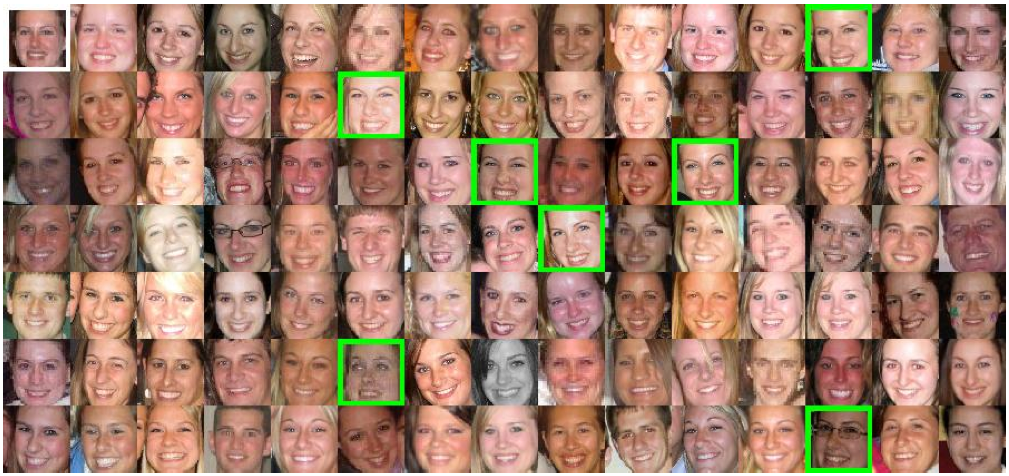
\includegraphics[width=3.5in]{ivw_facescores}
\end{center}
\vspace{-0.25in} \caption{\captionsize 
The performance of a commercial face recognition system on tagged faces harvested from Facebook~\cite{Stone2008}. Given the query face in the upper left, the system has returned the remaining faces as being most similar. Similarity to the query decreases from left to right and from top to bottom, and the ground-truth matches are highlighted with green squares. Due to the variability of this `real-world' dataset, the correct matches are not highly ranked.\label{fig:face-results}\afterfigspace}
\end{figure}



\SubSubSection{Preliminary Study}\label{sec:prelim-face-results}
Evidence for the utility of social network context is provided under simplified assumptions by the work of PI Zickler~\cite{Stone2008,Stone2010}, the former of which received the Best Paper Award at the First IEEE Workshop on Internet Vision. This work reported the results of a preliminary study on the ability of social network context to improve face-based identity recognition using a subset of 2641 labeled faces from Facebook. In this study, we restricted our attention to images with two faces (two-node graphs) so that CRF training and inference could be achieved without approximation. The label space ${\cal L}=\{l_0,\ldots,l_M\}$  consists of a set of possible identities, and we considered a simple set of individual node descriptions and contextual relationship descriptions. Specifically, we assumed that all descriptions in all views are observed and error-free, in which case the potentials in (\ref{eq:energy_simple}) are further expanded as a linear combination of view-specific univariate and bivariate \emph{feature functions} independent of observability variables $P,Q$:
\begin{eqnarray}
\phi_i(y_i|N,P) &=& \sum_{v_1} \alpha_{v_1}(N^{(v_1)}) f_{v_1}(y_i, N^{(v_1)})\\
\phi_{ij}(y_i, y_j|A,Q) &=& \sum_{v_2} \beta_{v_2}(A^{(v_2)}) g_{v_2}(y_i, y_j, A^{(v_2)}).
\end{eqnarray}


\begin{figure}[t!]
\begin{center}
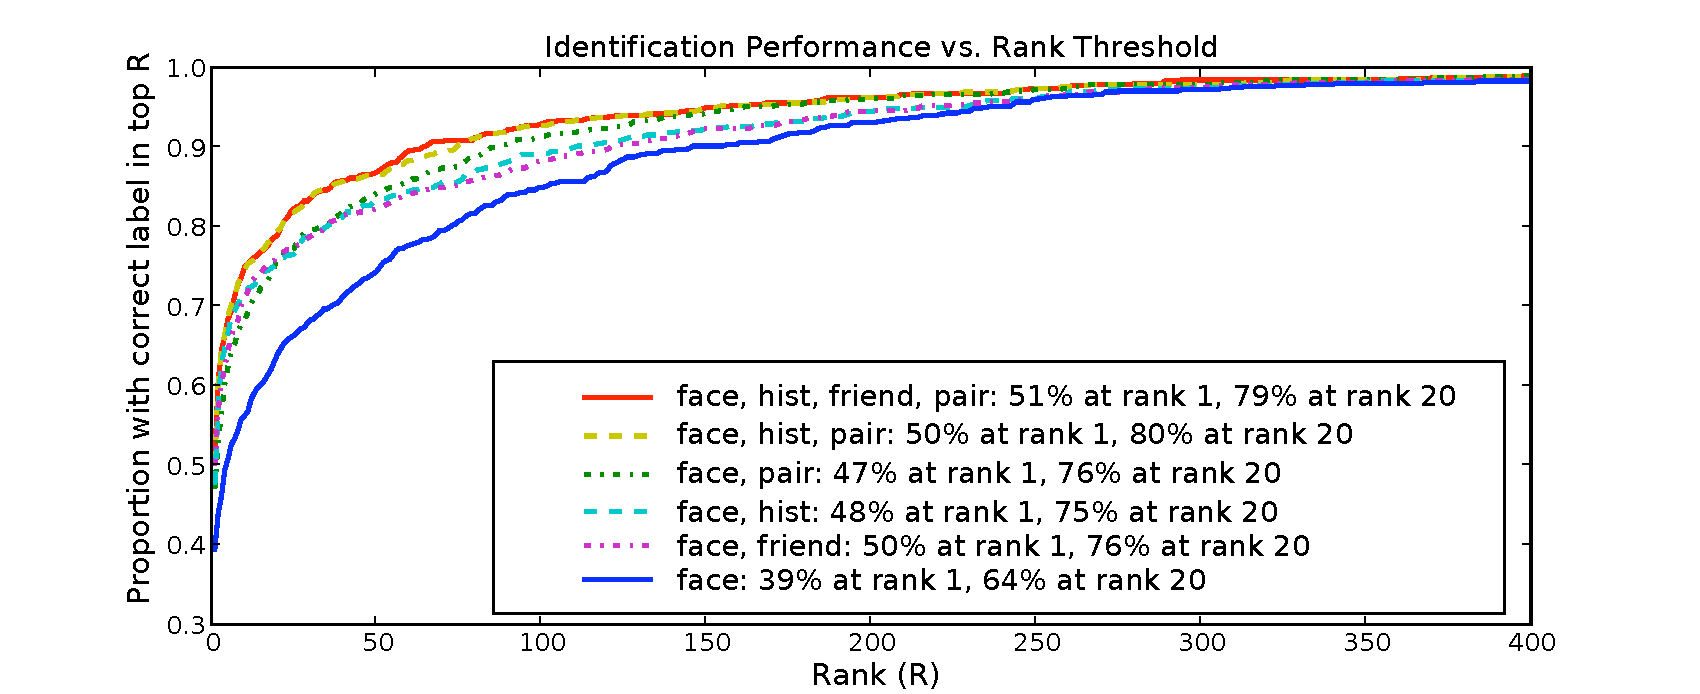
\includegraphics[width=5in]{rank_graph_small}\\
{\footnotesize
\begin{tabular}{ll}
\hline\hline\multicolumn{2}{l}{\raisebox{-0.1in}{Univariate Functions $f_{v_1}(y_i, N^{(v_1)})$}} \\
\hline
\parbox[t]{1.8in}{\raggedright Face score (\textsf{face})} & \parbox[t]{3.5in}{A distribution of likelihoods over ${\cal L}$ returned by a commercial face recognition system (see Fig.~\ref{fig:face-results})} \vspace{0.03in}\\
\parbox[t]{1.8in}{\raggedright Photo history (\textsf{hist})} & \parbox[t]{3.5in}{Number of times each individual $l_m$ has been tagged in previous photos posted by the photographer} \vspace{0.07in}\\
\multicolumn{2}{l}{Bivariate Functions $ g_{v_2}(y_i, y_j, A^{(v_2)})$} \\
\hline
\parbox[t]{1.8in}{\raggedright Friendship (\textsf{friend})}& \parbox[t]{3.5in}{Binary indicator that is one iff individuals $l_m$ and $l_n$ are `Facebook friends' } \vspace{0.04in}\\
\parbox[t]{1.8in}{\raggedright Pairwise co-occurrence (\textsf{pair})}& \parbox[t]{3.5in}{Number of times each pair of individuals $(l_m,l_n)$ has been jointly tagged in previous photos posted by the photographer}\\
\end{tabular}}
\end{center}
\captionspace \caption{\captionsize 
Face recognition performance as a function of rank threshold for a variety of combinations of feature functions (described bottom). At each rank value $R$, the graph displays the proportion of all test samples for which the correct ground-truth identity label appeared in the top $R$ predictions. Social network context improves recognition, and different sources of context information are complimentary\cite{Stone2008}.\label{fig:ivw-curves}\afterfigspace}
\end{figure}


The results are summarized in Figs.~\ref{fig:face-results} and \ref{fig:ivw-curves}. For each combination of feature functions, we determined model parameters ($\alpha$ and $\beta$) by maximizing the conditional log-likelihood of a training set by gradient ascent. Then, for each left-out test photo, exact marginal probabilities were computed for the test photo's face-nodes, and  the outputs were compared against ground truth. Specifically, the marginal probabilities were used to compute a ranked list at each node, and we measured how often the correct identity label appeared in the top $R$ ranks for a sliding value of $R$ (c.f.~\cite{frvt06}).

A number of observations can be drawn from these results. First, even when using the face score (\textsf{face}) alone (see Fig.~\ref{fig:face-results}) social network context plays a vital role. In our data, over 99\% of tagged faces correspond to `friends' of the photographer, and since the identity of the photographer is known (it is included in the input $N$), we can safely reduce the label space ${\cal L}$ from the 15,752 individuals in the global gallery to the hundreds of friends of the input photographer. Without this restriction, the results in Fig.~\ref{fig:face-results} would degrade remarkably. The results in Fig.~\ref{fig:ivw-curves} also demonstrate that social network context substantially improves baseline face recognition, and that different sources of context information are complementary.


These preliminary results are encouraging, especially since the network context information that was employed barely scratches the surface of possibilities. Existing work shows that clothing can provide useful information within an album~\cite{anguelov2007cir, zhang2003aah,  song2006cah, sivic2006fpr}, and it is possible that clothing could be used more globally as well, since the long-term clothing trends of certain individuals may be distinguishable from those of others. Recognition of facial attributes~\cite{LNCS53050340}, such as glasses or facial hair, can be used in conjunction with identity scores to improve recognition, and the same is true for gender recognition, which in many online communities is a knowable piece of information. In addition, people associate with each other in homes, schools, outdoors, workplaces, clubs, and so on, and a more explicit representation of these would be beneficial. Certain individuals will appear more often in certain types of scenes, and these `likely' scene types will change depending on who they are with. Temporal and geographic information, when available, may be further predictive of which individual is likely to occur and with whom. 



In our proposed research, we aim to both qualitatively and quantitatively analyze large collections of images and their embedding network to discover the utility of these multi-view context information, and in particular, explore effective approaches to account for incompletely observed graph, which is the crucial to allow our framework to succeed in realistic network conditions.